% Section 4: Results
% Source: context/Discussion_and_Conclusions.md §D2-D4, §D12
% Source: context/Paper_Layout_Plan.md §4
%
% EM-DASH PROHIBITION: Do not use --- or \textemdash. Use colons or semicolons.

\section{Empirical Study Results}\label{sec:results}

A total of 50{,}400 runs completed (48{,}000 at L2, the primary analysis
condition; 2{,}400 at L1). We report
results organised by research question.

\subsection{RQ1: Prevalence and Cross-Model Variation}\label{sec:rq1}

The pre-declared primary aggregate is pooled \DFR{} across all 16~models
at L2 (48{,}000 runs); the 15-model figure excluding the Mistral~Large~3
outlier is a pre-specified sensitivity check.

The overall JWT Defect/Failure Rate across 16 models under L2 conditions was
\textbf{18.0\%} (95\% CI: [17.6\%, 18.3\%]). Approximately one in six
authenticated tool-chain invocations produced a cryptographically invalid JWT.

Per-model \DFR{} ranged from \textbf{0.5\% to 99.8\%}
(Table~\ref{tab:failure_matrix}, Figure~\ref{fig:dfr_model}).
No model achieved zero \DFR{}.

\textbf{Outlier analysis: Mistral Large~3.}
Mistral Large~3 (99.8\% \DFR{}, 3{,}000 L2 runs) is qualitatively distinct.
Manual inspection of 50~outputs confirms explanation-mode semantic substitution
as the dominant failure (99.0\%): the model returns a description rather than
the credential. Two causes are consistent:
(i)~a \emph{tokenisation artifact} (aggressive BPE fragmentation favouring
paraphrase), or (ii)~a \emph{model-configuration artifact} (the pinned
version's instruction-following profile prioritising explanation).
The implication is that some models may be inherently unsuitable for direct
credential relay, strengthening the case for an architectural bypass. Excluding this outlier, pooled \DFR{} is
\textbf{12.5\%} (95\% CI: [12.2\%, 12.8\%], $N\!=\!45{,}000$, 15~models),
confirming that the headline finding is not driven by a single outlier.
BH-corrected pairwise Fisher's exact tests across all
$\binom{16}{2}\!=\!120$ model pairs found 110 of 120 pairs (92\%) significantly
different at $\alpha\!=\!0.05$, confirming near-universal heterogeneity.

\begin{figure}[t]
  \centering
  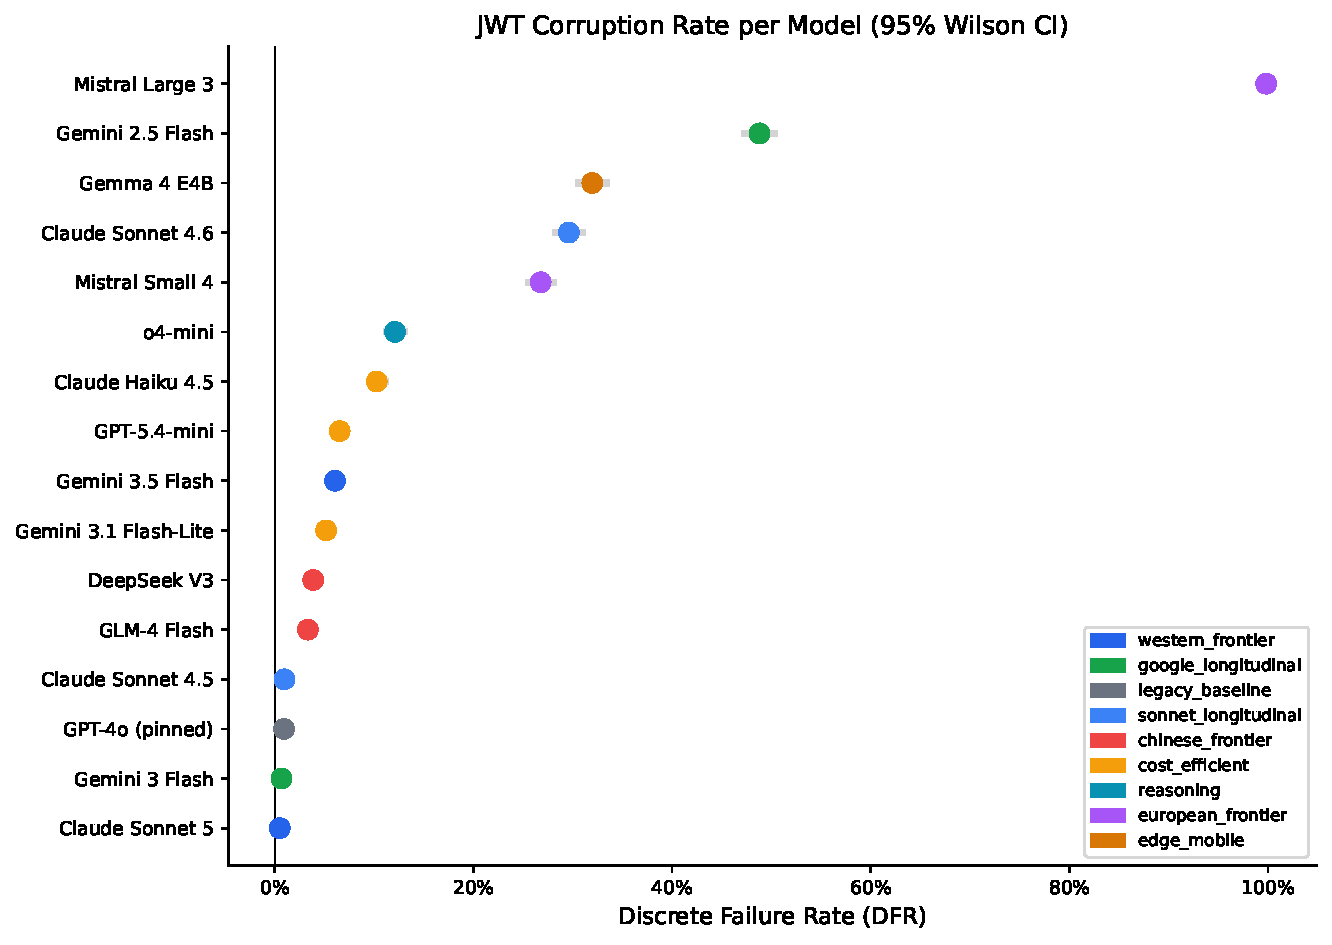
\includegraphics[width=0.82\columnwidth]{figures/fig01_dfr_by_model.pdf}
  \vspace{-4pt}\caption{Per-model JWT Defect/Failure Rate with Clopper-Pearson 95\%
  confidence intervals, sorted ascending and grouped by tier.}
  \label{fig:dfr_model}
\end{figure}

% Table 4: Per-model failure-type breakdown matrix
\begin{table*}[t]
\centering
\footnotesize
\vspace{-4pt}\caption{Per-model failure-type breakdown. Values are percentages of total L2 runs per model. \DFR{} = $1 -$ Exact Match \%.
Clopper-Pearson 95\% CIs reported for \DFR{} only.}
\label{tab:failure_matrix}
\begin{tabular}{@{}llrrrrrr@{}}
\toprule
\textbf{Model} & \textbf{Tier} & \textbf{Exact \%} & \textbf{Corrupt \%} & \textbf{Sem.Sub \%} & \textbf{Abst \%} & \textbf{DFR \%} & \textbf{95\% CI} \\
\midrule
% Data extracted from reports/parquet/main_l2.parquet (N=48,000 L2 runs)
% Sorted by DFR descending. Corrupt\% merges corrupted + truncated categories.
% Note: Refusal rate was 0.0\% for all 16 models and is omitted from this table.
Mistral Large 3          & EF & 0.2  & 0.0  & 99.0 & 0.8 & 99.8 & [99.6, 99.9] \\
Gemini 2.5 Flash         & GL & 51.2 & 48.7 & 0.0  & 0.1 & 48.8 & [47.0, 50.6] \\
Claude Sonnet 4.6        & SL & 70.4 & 0.6  & 28.0 & 1.0 & 29.6 & [28.0, 31.3] \\
Gemma 4 E4B              & LO & 68.0 & 28.9 & 1.4  & 1.7 & 32.0 & [30.3, 33.7] \\
Mistral Small 4          & EF & 73.2 & 22.4 & 4.2  & 0.2 & 26.8 & [25.2, 28.4] \\
\midrule
o4-mini                  & R  & 87.9 & 5.4  & 0.0  & 6.7 & 12.1 & [11.0, 13.3] \\
Claude Haiku 4.5         & CE & 89.7 & 10.0 & 0.3  & 0.0 & 10.3 & [9.2, 11.4] \\
GPT-5.4-mini             & CE & 93.5 & 6.5  & 0.0  & 0.0 & 6.5  & [5.7, 7.5] \\
Gemini 3.5 Flash         & WF & 93.9 & 5.2  & 0.0  & 0.9 & 6.1  & [5.2, 7.0] \\
Gemini 3.1 Flash-Lite    & CE & 94.8 & 0.4  & 4.7  & 0.0 & 5.2  & [4.4, 6.0] \\
\midrule
DeepSeek V3              & CF & 96.1 & 3.8  & 0.1  & 0.0 & 3.9  & [3.2, 4.6] \\
GLM-4 Flash              & CF & 96.7 & 1.8  & 0.0  & 1.6 & 3.3  & [2.7, 4.0] \\
Claude Sonnet 5          & WF & 99.5 & 0.5  & 0.0  & 0.0 & 0.5  & [0.3, 0.8] \\
Claude Sonnet 4.5        & SL & 99.0 & 1.0  & 0.0  & 0.0 & 1.0  & [0.6, 1.4] \\
GPT-4o (pin.)            & LB & 99.1 & 0.5  & 0.5  & 0.0 & 0.9  & [0.6, 1.3] \\
Gemini 3 Flash           & GL & 99.3 & 0.7  & 0.0  & 0.0 & 0.7  & [0.4, 1.0] \\
\midrule
\textbf{All models (N=48,000)} & & 82.0 & 8.5 & 8.6 & 0.8 & \textbf{18.0} & [17.6, 18.3] \\
\bottomrule
\end{tabular}
\end{table*}

No model exhibited safety-based refusal (0.0\%; see taxonomy,
Table~\ref{tab:taxonomy}). Cost-efficient models do not uniformly exhibit
higher \DFR{} than frontier models. The reasoning-tier model (o4-mini) shows a distinctive profile:
chain-of-thought inference fragments credentials through an additional
generation layer. Chinese frontier models show \DFR{} consistent with
different BPE vocabularies from Chinese-dominant corpora.

\subsection{RQ2: Structural Anatomy of Corruption}\label{sec:rq2}

\textbf{Length-gating.}
\DFR{} increases monotonically across tiers (Figure~\ref{fig:length_trend}):
short~12.6\%, medium-low~12.6\%, medium~13.6\%, long~22.2\%, very-long~28.7\%
(Spearman $\rho\!=\!0.900$, $p\!=\!0.037$). A Mantel-Haenszel test
(high tiers: long\,+\,very-long vs.\ low tiers: short\,+\,medium-low;
16~model strata) confirms a significant length effect:
OR~=~4.785 (95\% CI: [1.14, 20.0], $p\!<\!0.001$).
This result is identical when Mistral~Large~3 is excluded
(OR~=~4.785, 15~strata, $p\!<\!0.001$), confirming the length effect
is not an artefact of that single outlier.
Context depth DFR is monotonically increasing across three levels
($\rho\!=\!1.000$; $n\!=\!3$ precludes a meaningful permutation $p$-value);
A within-model GEE (groups\ =\ model, controlling for JWT length tier)
yields OR~=~1.093 (95\% CI: [0.84,~1.42], $p\!=\!0.51$), indicating no
statistically significant independent context effect once model identity
and token-length are held constant.

\begin{figure*}[t]
  \centering
  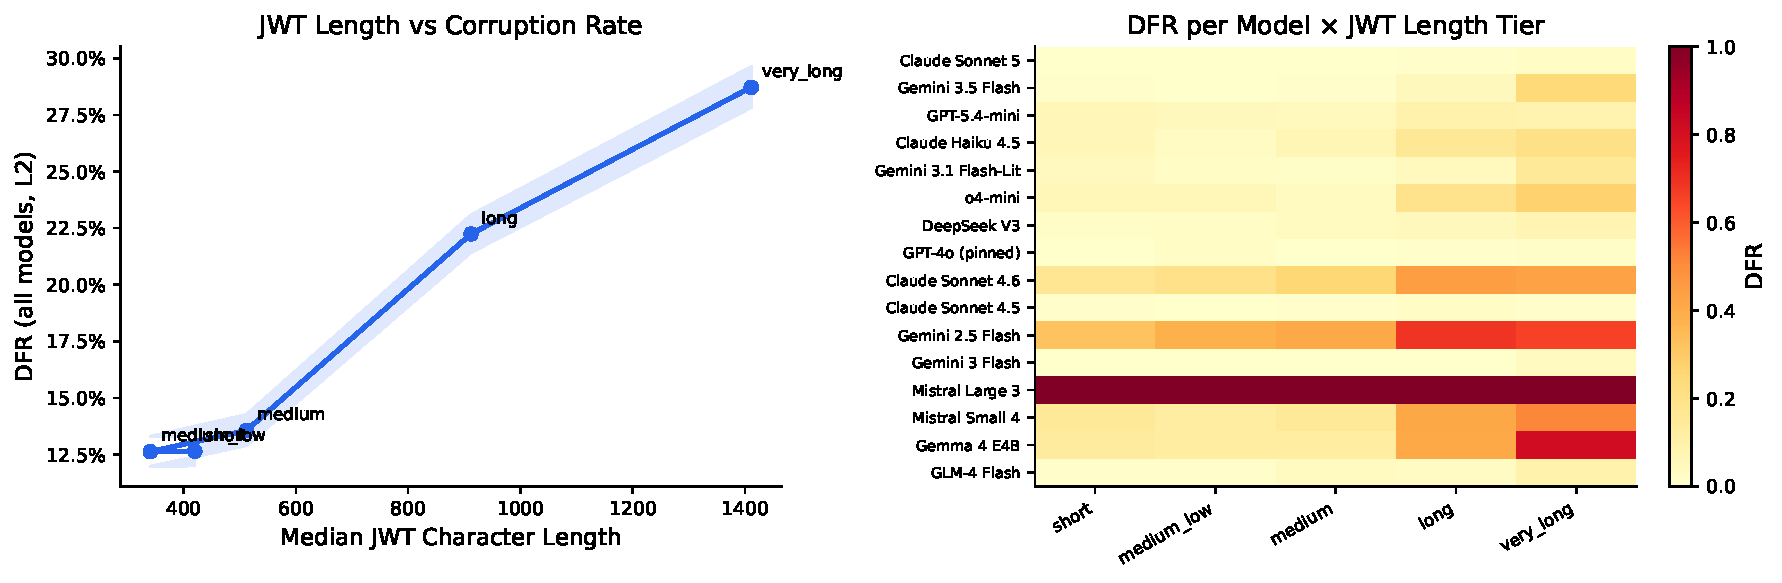
\includegraphics[width=0.82\textwidth]{figures/fig02_length_trend.pdf}
  \vspace{-4pt}\caption{\DFR{} by JWT length tier and context depth (left) and per-model
  \DFR{} heatmap across length tiers (right). The onset of non-trivial
  corruption occurs at $\sim$200 characters.}
  \label{fig:length_trend}
\end{figure*}

\textbf{Segment analysis.}
Segment Corruption Rate (SCR) analysis reveals that payload corruption dominates:
among character-level failures, 92.8\% involve payload mismatch, followed by
signature (11.3\%) and header (0.4\%). For the synthetic HS256 tokens used, the
payload is the longest Base64url segment; this segment-level length-gating mirrors
the JWT-level finding, consistent with BPE boundary exposure scaling with segment
length.
Among corrupted runs, 41.0\% show single-character substitution
(Levenshtein $L\!=\!1$) and 35.1\% show $L>5$ (mean $L\!=\!59.5$, pulled
upward by near-total rewrites), indicating a bimodal severity distribution.
DFR at fully deterministic sampling ($T\!=\!0.0$) was 17.3\%, only 1.3~pp
below $T\!=\!0.7$ (18.6\%), confirming the dominant failure mode is
deterministic, not sampling-noise-driven.

\textbf{Failure taxonomy.}
Table~\ref{tab:taxonomy} presents the six-outcome taxonomy (\Contrib{2}).
Character-level corruption (Levenshtein $\geq 1$, modal distance $L\!=\!1$) is
the dominant failure mode. Truncation (credential cut short) is a structurally
distinct sub-mode observed in 0.4\% of runs and reported merged with
\texttt{corrupted} in Table~\ref{tab:failure_matrix}. Semantic substitution,
where the LLM decodes the JWT payload and returns a plausible but
cryptographically invalid value, is rare but architecturally critical: it is
undetectable by any validation mechanism that does not hold a reference copy of
the original token.

\begin{table}[t]
\centering
\footnotesize
\vspace{-4pt}\caption{Six-outcome taxonomy of JWT relay results (\Contrib{2}). The
architectural implication column motivates the design decisions in
Section~\ref{sec:reference_architecture}. \texttt{refusal} had 0.0\%
observation rate in this study but is architecturally relevant
(Section~\ref{sec:ra_motivation}).}
\label{tab:taxonomy}
\begin{tabular}{@{}lp{4.5cm}@{}}
\toprule
\textbf{Outcome} & \textbf{Architectural Implication} \\
\midrule
\texttt{exact\_match}  & No intervention required \\
\texttt{corrupted}     & Interceptor must hold reference copy \\
\texttt{truncated}     & Credential shortened; same cryptographic impact as corrupted \\
\texttt{sem\_sub}      & Levenshtein detection insufficient; credential must not pass through LLM \\
\texttt{abstention}    & LLM cannot be relied upon for credential forwarding \\
\texttt{refusal}       & Out-of-band credential passing is the only solution \\
\bottomrule
\end{tabular}
\end{table}

\subsection{RQ3: Prompt Engineering as Insufficient Mitigation}\label{sec:rq3}

The L1$\rightarrow$L2 prompt transition produces a marginal, non-significant
change in overall \DFR{} ($+1.1$~pp, $p\!=\!0.18$), confirming that
increased instruction detail did not eliminate the observed corruption.

The ecological validity arm ($N\!=\!1{,}600$) provides the key measurement
under production conditions. Using the production \texttt{BearerTokenParam} instruction
(318~characters, explicitly naming the RSA signature consequence), the \DFR{}
was \textbf{19.9\%}. The difference from the main study at the same length tier
was $+1.9$~percentage points ($p\!=\!0.16$, Wilcoxon; not
significant). Spearman's rank correlation between eco arm and main experiment
model rankings was $\rho\!=\!0.740$ ($p\!=\!0.001$), confirming that model
rankings transfer to production conditions.

The most explicit instruction achievable within the MCP tool schema design space
produces a result statistically indistinguishable from neutral vocabulary.
Corruption persists regardless of prompt specificity; BPE tokenisation boundaries
appear to operate below the level of instruction-following behaviour and were not
overcome by any prompt tested in this study. We note that non-significance alone
does not constitute formal equivalence: establishing a true prompt ceiling would
require pre-specified equivalence margins and a TOST procedure, which is
identified as future work (Section~\ref{sec:conclusion}).
